\documentclass[11pt,a4paper]{article}

\usepackage[utf8]{inputenc}
\usepackage[T1]{fontenc}
\usepackage{amsmath,amssymb,amsthm}
\usepackage{mathtools}
\usepackage{booktabs}
\usepackage{hyperref}
\usepackage{geometry}
\usepackage{enumitem}
\usepackage{listings}
\usepackage{longtable}
\usepackage{textcomp}
\usepackage{array}
\usepackage{tikz}
\usetikzlibrary{arrows.meta,positioning,calc,shapes.geometric}

\geometry{margin=1in}
\setcounter{tocdepth}{2}

\newtheorem{definition}{Definition}[section]
\newtheorem{principle}[definition]{Principle}
\newtheorem{theorem}[definition]{Theorem}
\newtheorem{proposition}[definition]{Proposition}
\newtheorem{invariant}[definition]{Invariant}
\newtheorem{remark}[definition]{Remark}

\lstset{
  basicstyle=\ttfamily\small,
  columns=fullflexible,
  keepspaces=true,
  xleftmargin=2em,
  aboveskip=0.5em,
  belowskip=0.5em
}

\title{The Ledger Valuation Stack\\[6pt]
\large Pricing, Greeks, Continuous Approximate Pricing, and Temporal Orchestration\\[4pt]
\normalsize Companion Document to the Ledger Framework Specification}
\author{R.\ Delloye}
\date{March 2026 --- v0.1}

\begin{document}
\maketitle

\begin{abstract}
The Ledger framework~\cite{ledger} defines portfolio value as $V_t = \sum_u \mathrm{own}(u) \cdot P_t(u)$ and proves that PnL is path-independent: it depends only on the initial and final snapshots, not on intermediate trading activity.  The framework deliberately treats $P_t$ as an external input---``a function from units to prices in the reference currency''---without specifying how that function is computed, validated, or delivered.

This companion document fills the gap.  It defines the \emph{ValuationRecord}---a structured object that enriches the scalar price with Greeks, model provenance, market data lineage, and a quality flag---and shows that the path-independence theorem is preserved because the scalar \texttt{dirty\_price} field is precisely the $P_t(u)$ of the main framework.  It establishes that \emph{Greeks are model outputs, not instrument properties}: they are sensitivities of a specific model's price function to its inputs, and different models produce different Greeks for the same instrument and market data.  The \texttt{model\_id} field in the ValuationRecord is therefore load-bearing---it tells consumers which model's Greeks they are looking at.

It introduces the \emph{Pricing DAG}, the directed acyclic graph of dependencies between units and market data observables, specifying the construction algorithm that builds the DAG from unit store declarations and the mutation protocol that governs mid-cycle topology changes.  Temporal.io workflows implement reactive, DAG-driven pricing: one workflow per unit, upstream signals triggering downstream re-pricing, heterogeneous compute budgets, and stale-price policies.

A key architectural contribution is \emph{continuous approximate pricing}: between full reprices, every unit has an approximate price available via Taylor expansion from the last full valuation and cached Greeks plus current market moves.  At any time~$t$, a price is always available---either FIRM (full reprice, PnL explain passed), APPROXIMATE (Taylor expansion from last FIRM valuation), or STALE (last FIRM valuation older than the staleness threshold).

The document formalises PnL explain---the Taylor-expansion verification gate that every new valuation must pass before publication---connecting the multivariate polynomial analysis of~\cite{pnl_explain} to the operational pipeline.  Finally, it traces a complete valuation cycle through a three-instrument portfolio, showing every workflow signal, pricer invocation, PnL explain check, and publication step with concrete numbers.

The document is self-contained and independently readable.  It references the Ledger specification and the PnL explain paper by citation, not by import.
\end{abstract}

\tableofcontents
\clearpage

%==============================================================================
\section{Introduction}
\label{sec:intro}
%==============================================================================

The Ledger framework~\cite{ledger} establishes six properties by construction: atomicity, conservation, determinism, state-sufficiency, lifecycle value invariance, and time travel.  Portfolio valuation appears in~\cite[\S4]{ledger} as:
\[
V_t = \sum_{u \in \mathcal{U}} w_t(u) \cdot P_t(u)
\]
where $w_t(u)$ is the wallet balance (or, in the generalised position model, $\mathrm{own}(u)$) and $P_t(u)$ is the price of unit $u$ at time $t$ in the reference currency.  The path-independence theorem~\cite[\S4.3]{ledger} proves that $\mathrm{PnL} = V_{t_1} - V_{t_0}$ regardless of intermediate trading activity.

The framework is deliberately agnostic to the pricing methodology: ``$P_t$ is an \emph{external input} to the framework, not computed by it''~\cite[\S4.1]{ledger}.  This is the correct architectural boundary---the ledger is a settlement and position system, not a pricing engine.  But the boundary creates four unanswered questions:

\begin{enumerate}
\item \textbf{What does $P_t(u)$ return?}  In practice, a price is not a scalar.  A pricing computation produces sensitivities (Greeks), model provenance, market data lineage, compute time, and a quality assessment.  How does this structured output interact with the scalar $P_t$ of the PnL theorem?

\item \textbf{How are prices computed in dependency order?}  An NVDA vanilla call depends on NVDA spot, the NVDA implied volatility surface, and the USD risk-free rate curve.  A structured note embedding the call depends on the call's valuation.  How is this dependency graph defined, enforced, and executed?

\item \textbf{How are new prices validated before they enter the ledger's valuation store?}  The PnL explain analysis~\cite{pnl_explain} provides the mathematical foundation---Taylor expansion of price changes in terms of Greeks and market data moves---but does not specify the operational pipeline: when does the check run, what happens on failure, how does the system recover?

\item \textbf{What price is available between full reprices?}  Full repricing of complex instruments takes seconds to minutes.  Between pricing cycles, the risk pipeline needs a current price.  How is this provided?
\end{enumerate}

This document answers all four.

\subsection{Relationship to the Ledger Specification}

This document is a companion to, not a revision of, the Ledger framework~\cite{ledger}.  It introduces no new primitives (no new move types, no new wallet structures, no changes to the conservation law).  It specifies the \emph{valuation layer} that produces the $P_t$ function consumed by the ledger's PnL computation.  All definitions, notation, and conventions follow~\cite{ledger} unless stated otherwise.

\subsection{Relationship to the PnL Explain Paper}

The PnL explain paper~\cite{pnl_explain} establishes the mathematical foundation: for a pricing function $P$ approximated as a polynomial of degree three in the market data vector $x$, the price change decomposes as:
\[
P(x_2) - P(x_1) = \left\langle \frac{\Delta_{x_2} + \Delta_{x_1}}{2} \,\middle|\, x_2 - x_1 \right\rangle - \frac{1}{12}\langle x_2 - x_1 \,|\, (\Gamma_{x_2} - \Gamma_{x_1}) \,|\, x_2 - x_1 \rangle
\]
where $\Delta_x = \nabla P(x)$ is the gradient (delta vector) and $\Gamma_x = \nabla^2 P(x)$ is the Hessian (gamma matrix).  The paper distinguishes ex ante PnL (using only information at $x_1$) from ex post PnL (using information at both $x_1$ and $x_2$).  This document operationalises those results as a verification gate in the pricing pipeline, and extends them to provide continuous approximate pricing between full reprices.

\subsection{Document Roadmap}

Section~\ref{sec:valuation-record} defines the ValuationRecord.  Section~\ref{sec:greeks} specifies Greeks as model-dependent sensitivities and defines the Greeks structure by instrument class.  Section~\ref{sec:pricing-dag} introduces the Pricing DAG and its construction algorithm.  Section~\ref{sec:temporal} specifies the Temporal workflow architecture for reactive pricing.  Section~\ref{sec:pnl-explain} formalises PnL explain as a verification gate.  Section~\ref{sec:approx-pricing} introduces continuous approximate pricing via Taylor expansion.  Section~\ref{sec:valuation-store} describes the valuation store and its interaction with the ledger.  Section~\ref{sec:edge-cases} catalogues edge cases.  Section~\ref{sec:worked-example} traces a complete valuation cycle with concrete numbers.  Section~\ref{sec:conclusion} identifies open problems.

\clearpage
%==============================================================================
\section{The Valuation Record}
\label{sec:valuation-record}
%==============================================================================

The Ledger specification defines $P_t : \mathcal{U} \to \mathbb{R}$ as a scalar function.  In practice, the output of a pricing computation is richer.  We define the structured output and show that the scalar theorem is preserved.

\begin{definition}[Valuation Record]
\label{def:valuation-record}
A \emph{ValuationRecord} for unit $u$ at time $t$ is a tuple:
\begin{lstlisting}
ValuationRecord:
    unit_id:          UnitId
    timestamp:        Timestamp
    dirty_price:      Decimal       -- full market value including accrual
    clean_price:      Decimal       -- quoted price net of accrual
    accrued:          Decimal       -- dirty_price - clean_price
    greeks:           Greeks        -- model-specific sensitivity vector
    model_id:         String        -- which pricer produced this (load-bearing)
    market_data_snap: SnapshotId    -- which market data was used
    compute_ms:       Int           -- how long pricing took
    quality:          Quality       -- FIRM | INDICATIVE | APPROXIMATE
                                    --   | STALE | FAILED
\end{lstlisting}
\end{definition}

\noindent The fields serve distinct consumers:

\begin{itemize}[nosep]
\item \textbf{dirty\_price}: the scalar consumed by the ledger's PnL computation ($V_t = \sum \mathrm{own}(u) \cdot \texttt{dirty\_price}_t(u)$).
\item \textbf{clean\_price, accrued}: reporting fields for bond and loan instruments where market convention quotes a clean price.
\item \textbf{greeks}: the model-specific sensitivity vector consumed by PnL explain (Section~\ref{sec:pnl-explain}), continuous approximate pricing (Section~\ref{sec:approx-pricing}), and the risk pipeline.  These Greeks are properties of the \emph{(instrument, model, market data)} triple, not of the instrument alone (Section~\ref{sec:greeks}).
\item \textbf{model\_id}: identifies which pricing model produced this record.  This field is load-bearing: the Greeks are meaningless without knowing which model produced them.  The valuation store can hold multiple ValuationRecords per \texttt{(unit\_id, timestamp)}---one per model (Section~\ref{sec:valuation-store}).
\item \textbf{market\_data\_snap}: provenance for audit and model risk management.
\item \textbf{compute\_ms}: operational telemetry for capacity planning.
\item \textbf{quality}: a flag consumed by the risk pipeline, the continuous approximation service, and by the obligation-liveness executor~\cite[\S14.7]{ledger} when deciding whether to act on a valuation.
\end{itemize}

\begin{principle}[Scalar Compatibility]
\label{princ:scalar-compat}
The ValuationRecord enriches but does not replace the scalar price function.  The \texttt{dirty\_price} field IS the $P_t(u)$ of~\cite[\S4.1]{ledger}.  The path-independence theorem~\cite[\S4.3]{ledger} is preserved:
\[
\mathrm{PnL} = V_{t_1} - V_{t_0} = \sum_{u} \mathrm{own}(u) \cdot \bigl[\texttt{dirty\_price}_{t_1}(u) - \texttt{dirty\_price}_{t_0}(u)\bigr]
\]
The remaining fields are metadata that enriches the record without altering the theorem.  No downstream consumer that depends on the scalar $P_t$ needs modification.
\end{principle}

\subsection{Quality Semantics}

The \texttt{quality} flag has five values with precise operational semantics:

\begin{center}
\small
\begin{tabular}{l p{9cm}}
\toprule
\textbf{Quality} & \textbf{Semantics} \\
\midrule
\texttt{FIRM} & Full reprice from live market data within the unit's cadence window; PnL explain passed.  This is the normal state. \\
\texttt{INDICATIVE} & Full reprice completed but PnL explain tolerance exceeded, or market data is from a secondary source.  Risk pipeline treats with elevated scrutiny. \\
\texttt{APPROXIMATE} & Taylor expansion from the last FIRM valuation using cached Greeks and current market data moves.  Available instantly between full reprices.  Not used for official PnL (Section~\ref{sec:approx-pricing}). \\
\texttt{STALE} & Last FIRM valuation is older than the staleness threshold.  The \texttt{timestamp} field shows when the price was last computed, not the current time. \\
\texttt{FAILED} & The pricer failed to produce any price.  No dirty\_price is available; downstream consumers use the previous FIRM price with STALE quality. \\
\bottomrule
\end{tabular}
\end{center}

\noindent The quality flag is consumed by three downstream systems.  The risk pipeline uses it for limit monitoring: a position valued at STALE triggers a staleness alert and may receive a prudential haircut; a position valued at APPROXIMATE is acceptable for intraday risk but not for end-of-day limits.  The obligation-liveness executor~\cite[\S14.7]{ledger} uses it for margin calculations: a CSA VM call computed on STALE valuations is flagged for manual review before dispatch.  The continuous approximation service (Section~\ref{sec:approx-pricing}) uses it to determine whether a Taylor expansion is valid (only from FIRM base valuations).

\subsection{Dirty Price, Clean Price, and Accrued Interest}

For instruments with accrual mechanics (bonds, loans, swaps with accrued interest), the \texttt{dirty\_price} is the economically complete price:
\[
\texttt{dirty\_price} = \texttt{clean\_price} + \texttt{accrued}
\]
The clean price is the market-quoted price excluding interest that has accrued since the last coupon date.  The accrued interest is computed from the unit state~\cite[\S7]{ledger}, which records the last coupon date, the coupon rate, and the day-count convention.  This is consistent with~\cite[\S5.3]{ledger}: ``the bond's price function $P_t(u)$ returns the \emph{dirty} price.''

For instruments without accrual (equities, cash, most derivatives), \texttt{clean\_price} $=$ \texttt{dirty\_price} and \texttt{accrued} $= 0$.

\clearpage
%==============================================================================
\section{Greeks as Model-Dependent Sensitivities}
\label{sec:greeks}
%==============================================================================

\subsection{Greeks Are Model Outputs}

A widespread but incorrect mental model treats Greeks as properties of an instrument---as if ``the delta of this call is 0.57'' were an objective fact like ``the strike of this call is 900.''  It is not.

\begin{principle}[Model Dependence of Greeks]
\label{princ:greeks-model-dep}
Greeks are sensitivities of a \emph{model's price function} to its inputs.  They are properties of the triple $(\text{instrument},\; \text{model},\; \text{market data})$, not of the instrument alone.  Formally, for a pricing model $\mathcal{M}$ that maps market data $x$ to a price $P_\mathcal{M}(x)$:
\begin{align}
\delta_\mathcal{M} &= \frac{\partial P_\mathcal{M}}{\partial S} &\quad&\text{(delta: sensitivity to underlying price)} \\[4pt]
\Gamma_\mathcal{M} &= \frac{\partial^2 P_\mathcal{M}}{\partial S^2} &\quad&\text{(gamma: convexity in underlying price)} \\[4pt]
\nu_\mathcal{M} &= \frac{\partial P_\mathcal{M}}{\partial \sigma_\mathcal{M}} &\quad&\text{(vega: sensitivity to the model's vol parameter)}
\end{align}
The subscript $\mathcal{M}$ is essential.  Different models produce different Greeks for the same instrument and the same market data.  This is not a bug---it is a fact about models.
\end{principle}

\paragraph{Illustrative example: delta of a vanilla call.}  Consider an at-the-money NVDA call with $S = K = 900$, $T = 0.25$, $r = 5\%$, and a market-observed implied volatility of 42\%.

\begin{itemize}[nosep]
\item \textbf{Black-Scholes} (flat vol): $\delta_{\mathrm{BS}} = N(d_1)$.  The model assumes a flat, constant volatility surface.  A single implied vol number parameterises the entire surface.
\item \textbf{Local volatility} (Dupire): $\delta_{\mathrm{LV}}$ is computed from the full local vol surface $\sigma_{\mathrm{loc}}(S, t)$.  The delta is typically lower than Black-Scholes for the same market conditions because the model captures the skew: as $S$ increases, local vol decreases (for typical equity skew), partially offsetting the price increase.
\item \textbf{Stochastic volatility} (Heston, SABR): $\delta_{\mathrm{SV}}$ accounts for the correlation between spot and vol dynamics.  With negative spot-vol correlation (typical for equities), the delta lies between BS and local vol.
\end{itemize}

\noindent The differences are material.  For a 25-delta put on a short-dated equity index option, the delta difference between Black-Scholes and a calibrated SABR model can be 2--5 delta points---significant for hedging.

\paragraph{Vega is particularly model-dependent.}  Black-Scholes vega assumes a flat vol surface shifts uniformly: $\nu_{\mathrm{BS}} = \partial P / \partial \sigma_{\mathrm{flat}}$.  But in practice, the vol surface has skew (across strikes) and term structure (across expiries).  ``Vega'' means different things depending on what is being bumped:
\begin{itemize}[nosep]
\item \emph{Parallel vega}: the entire surface shifts by $+1$~vol point.  This is Black-Scholes vega.
\item \emph{Bucket vega by expiry}: the surface shifts at one maturity pillar.
\item \emph{Bucket vega by strike}: the surface shifts at one strike pillar.
\item \emph{Bucket vega by both}: the surface shifts at one (strike, expiry) node.
\end{itemize}
The per-unit ValuationRecord's \texttt{model\_id} field tells consumers which of these conventions applies.

\subsection{Consequences for the Valuation Record}

The model dependence of Greeks has three operational consequences:

\begin{enumerate}
\item \textbf{The \texttt{model\_id} field is load-bearing.}  It is not audit metadata---it is required to interpret the Greeks.  A consumer who reads $\delta = 0.57$ without knowing the model cannot use the number for hedging, risk, or PnL explain.

\item \textbf{Multiple records per (unit, timestamp).}  The valuation store's primary key is \texttt{(unit\_id, timestamp, model\_id)}, not \texttt{(unit\_id, timestamp)}.  A single unit at a single timestamp may have ValuationRecords from multiple models.  This supports firms that run Greeks from multiple models and take the most conservative hedge or a weighted blend.

\item \textbf{PnL explain must be model-consistent.}  The Taylor expansion that verifies a new price must use the \emph{same model's} Greeks as the full reprice.  Concretely: if the previous FIRM record was produced by model $\mathcal{M}_1$ and the new candidate record is also from $\mathcal{M}_1$, the PnL explain uses $\mathcal{M}_1$'s Greeks.  Mixing models---e.g., explaining a local vol price change using Black-Scholes Greeks---will produce spurious unexplained PnL that is a model artefact, not a market signal.
\end{enumerate}

\subsection{Bump-and-Revalue vs.\ Analytical Greeks}

Most Greeks in practice are computed by \emph{bump-and-revalue}: perturb an input, reprice, and compute the finite difference:
\[
\delta \approx \frac{P(S + \epsilon) - P(S - \epsilon)}{2\epsilon}
\]
Only a few models (Black-Scholes for vanilla options, bond duration from cash flows) have closed-form Greeks.  The implications:

\begin{itemize}[nosep]
\item \textbf{Compute cost.}  Each first-order Greek requires 2 pricing calls (central difference) or 1 (forward difference).  Each cross-Greek (vanna, volga) requires 4 calls.  A full Greek computation for a five-factor instrument requires 10--20 additional pricing calls.  For a Monte Carlo pricer at 10 seconds per call, the full Greek computation takes 2--4 minutes.
\item \textbf{Temporal workflow implication.}  Greek computation is a separate activity from the base price activity, with its own timeout.  The PricingWorkflow first obtains the base price, then dispatches Greek computation as a parallel fan-out of bump-and-revalue activities.  If Greek computation times out, the base price is still published (with \texttt{quality = INDICATIVE} and empty Greeks), and Greek computation is retried in the background.
\item \textbf{Bump size matters.}  The bump $\epsilon$ must be chosen to balance truncation error (too large) against numerical noise (too small).  The bump size is model-specific and recorded in the ValuationRecord metadata.
\end{itemize}

\subsection{Greeks Structures by Instrument Class}

The \texttt{greeks} field of the ValuationRecord is a tagged union whose active variant depends on the instrument class.  This reflects the reality that different instruments have different risk factors.

\begin{definition}[Greeks]
\label{def:greeks}
The Greeks structure is an instrument-class-specific sensitivity vector:
\begin{lstlisting}
Greeks = EquityGreeks | OptionGreeks | ExoticOptionGreeks
       | IRSGreeks | BondGreeks | FuturesGreeks | CashGreeks
\end{lstlisting}
Each variant carries sensitivities of the \emph{specific model} identified by \texttt{model\_id}.
\end{definition}

\subsubsection{Equity Greeks}

\begin{lstlisting}
EquityGreeks:
    delta:    Decimal = 1.0    -- dP/dS; always 1.0 for a spot position
\end{lstlisting}

\noindent An equity spot position has delta of exactly 1.0 by definition: a \$1 move in the spot price changes the position value by \$1 per share.  All higher-order sensitivities are zero.  This is the one case where Greeks are model-independent: the ``model'' is the identity function $P(S) = S$.

\subsubsection{Vanilla Option Greeks}

\begin{lstlisting}
OptionGreeks:
    delta:    Decimal    -- dP/dS
    gamma:    Decimal    -- d^2P/dS^2
    vega:     Decimal    -- dP/d(sigma_M)  [model-specific vol parameter]
    theta:    Decimal    -- dP/dt (per calendar day)
    rho:      Decimal    -- dP/dr
\end{lstlisting}

\noindent These are the five first- and second-order sensitivities.  The subscript on $\sigma_\mathcal{M}$ is suppressed in the field name for readability, but the model dependence is real: for Black-Scholes, $\sigma$ is flat implied vol; for local vol, it is the ATM local vol; for SABR, it is the $\alpha$ parameter.  The \texttt{model\_id} field on the enclosing ValuationRecord disambiguates.

\subsubsection{Exotic Option Greeks}

\begin{lstlisting}
ExoticOptionGreeks:
    delta:    Decimal    -- dP/dS
    gamma:    Decimal    -- d^2P/dS^2
    vega:     Decimal    -- dP/d(sigma_M)
    theta:    Decimal    -- dP/dt
    rho:      Decimal    -- dP/dr
    vanna:    Decimal    -- d^2P/(dS d(sigma_M))
    volga:    Decimal    -- d^2P/d(sigma_M)^2
    charm:    Decimal    -- d^2P/(dS dt)
\end{lstlisting}

\noindent Exotic options (barriers, Asians, lookbacks) require cross-sensitivities for accurate PnL explain.  Vanna captures the sensitivity of delta to volatility, volga captures the convexity of price with respect to volatility, and charm captures the time-decay of delta.  These are almost always computed by bump-and-revalue: closed-form cross-Greeks exist only for Black-Scholes on vanillas.

\subsubsection{Interest Rate Swap Greeks}

\begin{lstlisting}
IRSGreeks:
    dv01:               Decimal    -- dollar value of one basis point
    convexity:          Decimal    -- second-order rate sensitivity
    key_rate_durations: Map<Tenor, Decimal>  -- per-tenor DV01
\end{lstlisting}

\noindent For an IRS, the risk factor is the yield curve, not a single spot price.  DV01 is the change in present value for a one-basis-point parallel shift; key-rate durations decompose this sensitivity across tenors (1y, 2y, 5y, 10y, 30y, etc.).  The PnL explain for an IRS uses:
\[
\text{explained PnL} \approx \sum_{\tau} \mathrm{KRD}_\tau \cdot \Delta r_\tau + \frac{1}{2} \cdot \mathrm{convexity} \cdot (\Delta r_{\text{par}})^2
\]
where $\Delta r_\tau$ is the change in the zero rate at tenor $\tau$.  The curve bootstrapping model (e.g., cubic spline vs.\ piecewise linear) affects the key-rate durations---another instance of model dependence.

\subsubsection{Bond Greeks}

\begin{lstlisting}
BondGreeks:
    modified_duration:  Decimal    -- -(1/P)(dP/dy)
    convexity:          Decimal    -- (1/P)(d^2P/dy^2)
    dv01:               Decimal    -- dollar value of one basis point
\end{lstlisting}

\noindent Bond Greeks are expressed in yield-to-maturity space.  Modified duration and convexity drive the PnL explain:
\[
\frac{\Delta P}{P} \approx -D_{\mathrm{mod}} \cdot \Delta y + \frac{1}{2} \cdot C \cdot (\Delta y)^2
\]

\subsubsection{Futures Greeks}

\begin{lstlisting}
FuturesGreeks:
    delta:              Decimal = 1.0    -- by definition
    accumulated_vm:     Decimal          -- variation margin to date
\end{lstlisting}

\noindent A futures contract has delta of 1.0 to its settlement price.  The \texttt{accumulated\_vm} field records the cumulative variation margin, connecting to the daily settlement workflow~\cite[\S14.4.1]{ledger}.

\subsubsection{Cash Greeks}

\begin{lstlisting}
CashGreeks:
    -- empty: no sensitivities for the reference currency
\end{lstlisting}

\noindent The reference currency (e.g., USD) has $P_t(\mathrm{USD}) = 1$ by definition.  Foreign currencies have an FX delta relative to the reference currency, modelled as an EquityGreeks with delta equal to the FX rate.

\subsection{Greeks for Risk Management: Multiple Models}

Firms typically run Greeks from multiple models for the same instrument:

\begin{itemize}[nosep]
\item A \emph{primary model} (e.g., calibrated local vol) for hedging and official PnL.
\item A \emph{secondary model} (e.g., SABR) for model risk assessment.
\item A \emph{stress model} (e.g., Black-Scholes with shocked vol) for regulatory capital.
\end{itemize}

\noindent The valuation store holds one ValuationRecord per (unit, timestamp, model), so all three sets of Greeks coexist.  The risk pipeline queries by model: hedging uses the primary model's delta; the model risk report compares all three.  When Greeks from multiple models disagree materially, the conservative choice (largest absolute delta for hedging, largest VaR for capital) is the standard practice.

\clearpage
%==============================================================================
\section{The Pricing DAG}
\label{sec:pricing-dag}
%==============================================================================

Pricing is not a flat operation over independent instruments.  The price of an NVDA vanilla call depends on NVDA spot, the NVDA implied volatility surface, and the USD risk-free rate curve.  A structured note embedding the call depends on the call's valuation.  These dependencies form a directed acyclic graph---the \emph{Pricing DAG}.

\subsection{Definition}

\begin{definition}[Pricing DAG]
\label{def:pricing-dag}
The \emph{Pricing DAG} is a directed acyclic graph $G = (N, E)$ where:
\begin{itemize}[nosep]
\item $N = N_U \cup N_M$: nodes are either unit nodes ($N_U \subseteq \mathcal{U}$, the units requiring valuation) or market data nodes ($N_M$, observable data feeds such as spot prices, yield curves, volatility surfaces).
\item $E \subseteq N \times N$: a directed edge $(a, b) \in E$ means ``$b$ requires a fresh price or data point from $a$ before it can be priced.''
\end{itemize}
\end{definition}

\noindent Market data nodes are leaf nodes (no incoming edges): they receive prices from external data feeds.  Equity spot positions are also near-leaf: they depend on a single market data node (the exchange price feed).  Derivatives and structured products are interior or root nodes with dependencies on both market data and other unit nodes.

\subsection{Construction Algorithm}
\label{sec:dag-construction}

The DAG is not manually specified.  It is constructed algorithmically from the unit definitions in the Unit Store~\cite[\S3]{ledger}.

\begin{definition}[DAG Construction]
\label{def:dag-construction}
\begin{lstlisting}
BuildPricingDAG(unit_store: UnitStore) -> DAG:
    dag = empty DAG

    -- Step 1: Add market data nodes (leaf nodes)
    for each observable o referenced by any unit in unit_store:
        dag.add_node(o, type=MARKET_DATA, dependencies=[])

    -- Step 2: Add unit nodes with dependencies
    for each unit u in unit_store where u.lifecycle_stage == ACTIVE:
        deps = u.smart_contract.pricing_dependencies()
        dag.add_node(u, type=UNIT, dependencies=deps)

    -- Step 3: Verify acyclicity
    if dag.has_cycle():
        raise DAGCycleError(dag.find_cycle())

    -- Step 4: Compute topological order
    dag.topo_order = topological_sort(dag)

    return dag
\end{lstlisting}
\end{definition}

\paragraph{The \texttt{pricing\_dependencies()} method.}  This is a method on the smart contract, declared at unit registration~\cite[\S3.4]{ledger}.  It returns the set of observables and other units that the instrument's price depends on.  Examples:

\begin{center}
\small
\begin{tabular}{l p{8cm}}
\toprule
\textbf{Instrument} & \textbf{\texttt{pricing\_dependencies()}} \\
\midrule
Vanilla option on NVDA & \texttt{\{NVDA\_spot, NVDA\_vol\_surface, USD\_rate\_curve\}} \\
Fixed-rate bond & \texttt{\{issuer\_yield\_curve\}} \\
IRS & \texttt{\{USD\_deposit\_rates, USD\_futures, USD\_swap\_rates\}} (or equivalently \texttt{\{USD\_yield\_curve\}}) \\
Structured note embedding NVDA call & \texttt{\{NVDA\_call\_unit, issuer\_credit\_curve\}} \\
Equity spot & \texttt{\{NVDA\_exchange\_price\_feed\}} \\
\bottomrule
\end{tabular}
\end{center}

\paragraph{Topological order determines evaluation sequence.}  The topological sort produces a linear ordering of nodes such that every node appears after all its dependencies.  Leaf nodes (market data) come first, then level-1 dependents (equity spot), then level-2 (vanilla options), then level-3+ (structured notes).  Each level can be evaluated in parallel: all nodes at the same level are independent of each other.

\begin{invariant}[Acyclicity]
\label{inv:acyclicity}
The Pricing DAG is acyclic.  This invariant is enforced at unit registration~\cite[\S3.4]{ledger}: the Unit Store rejects a unit whose pricing dependencies would create a cycle.
\end{invariant}

\noindent Acyclicity ensures that a topological ordering exists, guaranteeing that every unit can be priced after all its dependencies.  In practice, cycles are rare in financial instrument pricing (a call on NVDA does not have NVDA depending on the call), but the invariant prevents pathological configurations such as circular structured notes.

\subsection{DAG Topology by Instrument Class}

\begin{center}
\small
\begin{tabular}{l l l}
\toprule
\textbf{Instrument} & \textbf{Upstream dependencies} & \textbf{DAG depth} \\
\midrule
Cash (USD) & None & 0 (by definition) \\
Equity spot (NVDA) & NVDA exchange price feed & 1 \\
Vanilla option (NVDA call) & NVDA spot, NVDA vol surface, USD rate curve & 2 \\
Exotic option (barrier) & NVDA spot, NVDA vol surface, USD rate curve & 2 \\
IRS & USD yield curve (deposits, futures, swaps) & 2 \\
Bond & Issuer yield curve, USD rate curve & 2 \\
Structured note & Embedded option valuation, issuer credit curve & 3+ \\
\bottomrule
\end{tabular}
\end{center}

\subsection{Example: Three-Instrument Portfolio}

Figure~\ref{fig:pricing-dag} illustrates the Pricing DAG for the worked example in Section~\ref{sec:worked-example}: a portfolio containing NVDA spot, an NVDA Jun~2026 900~Call, and a structured note embedding the call.

\begin{figure}[ht]
\centering
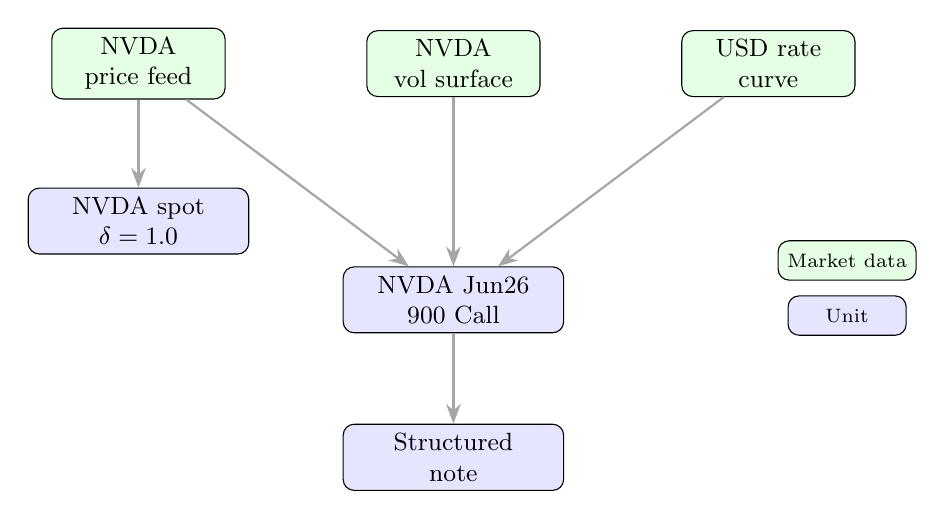
\begin{tikzpicture}[
    mkt/.style={draw, rounded corners, fill=green!10, minimum width=2.2cm, minimum height=0.8cm, font=\small, align=center},
    unit/.style={draw, rounded corners, fill=blue!10, minimum width=2.8cm, minimum height=0.8cm, font=\small, align=center},
    arr/.style={-{Stealth[length=2.5mm]}, thick, color=gray!70},
  ]
  % Market data nodes (leaves)
  \node[mkt] (spot_feed) at (0, 4)   {NVDA\\price feed};
  \node[mkt] (vol_surf)  at (4, 4)   {NVDA\\vol surface};
  \node[mkt] (rate)      at (8, 4)   {USD rate\\curve};

  % Unit nodes
  \node[unit] (nvda_spot) at (0, 2)   {NVDA spot\\$\delta = 1.0$};
  \node[unit] (nvda_call) at (4, 1)   {NVDA Jun26\\900 Call};
  \node[unit] (struct)    at (4, -1)  {Structured\\note};

  % Edges
  \draw[arr] (spot_feed) -- (nvda_spot);
  \draw[arr] (spot_feed) -- (nvda_call);
  \draw[arr] (vol_surf)  -- (nvda_call);
  \draw[arr] (rate)      -- (nvda_call);
  \draw[arr] (nvda_call) -- (struct);

  % Legend
  \node[mkt, minimum width=1.5cm, minimum height=0.5cm, font=\scriptsize] at (9, 1.5) {Market data};
  \node[unit, minimum width=1.5cm, minimum height=0.5cm, font=\scriptsize] at (9, 0.8) {Unit};
\end{tikzpicture}
\caption{Pricing DAG for the three-instrument portfolio.  Green nodes are market data feeds (leaf nodes); blue nodes are units requiring valuation.  Edges point from dependency to dependent.  NVDA spot depends only on its price feed.  The NVDA call depends on NVDA spot (via the price feed), the vol surface, and the rate curve.  The structured note depends on the call's valuation.}
\label{fig:pricing-dag}
\end{figure}

\subsection{DAG Mutation}
\label{sec:dag-mutation}

The Pricing DAG is not static.  It changes when units are added or removed.

\paragraph{New unit registered.}  Add the new node and its edges to the DAG.  Recompute the topological order.  Verify acyclicity---if the new unit's dependencies create a cycle, the registration is rejected~\cite[\S3.4]{ledger}.

\paragraph{Unit terminated.}  Remove the unit node and its edges.  Recompute the topological order.  Downstream dependents are notified that the dependency no longer exists; the terminated unit's terminal value (which is deterministic) is used.

\paragraph{Market data source switched.}  The market data node's identity changes, but the topology is preserved.

\paragraph{Mid-cycle mutation.}  The current pricing cycle completes with the old DAG.  The new DAG takes effect on the next cycle.  This ensures that a single cycle always operates on a consistent, frozen topology.  A new unit added mid-cycle will be priced on the next cycle, not retroactively inserted into the current one.

\noindent The DAG is rebuilt only when topology changes (unit registration, termination).  It is NOT rebuilt on every pricing cycle.

\clearpage
%==============================================================================
\section{Temporal Workflow Architecture for Pricing}
\label{sec:temporal}
%==============================================================================

The Ledger specification uses Temporal.io as its execution engine~\cite[\S14]{ledger}: lifecycle events, settlement, and obligation monitoring are orchestrated as Temporal workflows.  The valuation stack extends this architecture with pricing-specific workflows that implement the reactive, DAG-driven pricing pattern.

\subsection{Design Principle: One Workflow per Unit}

Each unit in the Pricing DAG has a dedicated \texttt{PricingWorkflow(unit\_id)} that:
\begin{enumerate}[nosep]
\item waits for all upstream dependencies to signal fresh prices,
\item retrieves market data,
\item invokes the pricer activity (base price),
\item dispatches Greek computation activities (bump-and-revalue fan-out),
\item runs PnL explain verification,
\item publishes the ValuationRecord,
\item updates the approximation service with fresh Greeks (Section~\ref{sec:approx-pricing}).
\end{enumerate}

This is a one-to-one mapping: every unit node in the Pricing DAG corresponds to exactly one long-running Temporal workflow.  The workflow is instantiated at unit registration and completed at maturity or termination, mirroring the lifecycle workflows of~\cite[\S14.4]{ledger}.

\subsection{Cadence and Heterogeneous Compute}

Different instruments require different pricing frequencies and have different compute budgets:

\begin{center}
\small
\begin{tabular}{l r r l}
\toprule
\textbf{Instrument class} & \textbf{Cadence} & \textbf{Compute budget} & \textbf{Pricer type} \\
\midrule
Equity spot & 1--5s & $< 1$ms & Trivial (pass-through) \\
Vanilla option & 10--30s & 1--10ms & Analytical (Black-Scholes) \\
Exotic option & 1--5min & 1--30s & Monte Carlo / PDE \\
IRS & 30s--2min & 10--100ms & Curve bootstrapping \\
Bond & 30s--2min & 1--10ms & Yield-to-maturity \\
Structured note & 5--15min & 1--60s & Composite (depends on embedded) \\
\bottomrule
\end{tabular}
\end{center}

\noindent The cadence is a configurable parameter on each PricingWorkflow, not a global constant.  Liquid equities may be priced every second; illiquid OTC exotics may be priced every 15 minutes or only on demand.

\subsection{Greek Computation as Separate Activity}

Greek computation is factored out of the base pricing activity because:
\begin{enumerate}[nosep]
\item It costs 10--50$\times$ the base price computation (bump-and-revalue for each risk factor).
\item It can time out independently---the base price should still be published even if Greek computation is slow.
\item The bump-and-revalue calls for different risk factors are independent and can run in parallel.
\end{enumerate}

\noindent The PricingWorkflow dispatches Greek computation as a fan-out of activities after the base price is obtained.  Each bump direction is an independent activity with its own timeout.  If Greek computation partially succeeds (e.g., delta and gamma computed but vega timed out), the available Greeks are published and the missing ones are retried.

\subsection{DAG Signalling}

The reactive pricing pattern is implemented through Temporal signals:

\begin{enumerate}[nosep]
\item When a leaf node (e.g., NVDA price feed) produces a new data point, it signals all downstream unit workflows that depend on it.
\item When a unit workflow produces a new ValuationRecord, it signals all downstream unit workflows that depend on it.
\item A downstream workflow maintains a freshness map: \texttt{Map<DependencyId, Timestamp>}.  When a signal arrives, the map is updated.  The workflow checks: ``do I have fresh prices for ALL my upstream nodes?''  If yes, fire pricing.  If not, wait.
\end{enumerate}

\noindent This is a data-flow / reactive pattern.  It has two key properties:

\begin{itemize}[nosep]
\item \textbf{No redundant computation.}  A workflow does not re-price until all upstream dependencies have refreshed.  If NVDA spot updates but the vol surface has not, the call's workflow waits.
\item \textbf{Automatic cascade.}  When the NVDA call produces a new ValuationRecord, it signals the structured note workflow, which then re-prices.  The cascade propagates through the DAG without explicit orchestration.
\end{itemize}

\subsection{Workflow Pseudocode}

\begin{lstlisting}
PricingWorkflow(unit_id, cadence, dependencies):
    prev_record = None
    freshness = {dep: None for dep in dependencies}
    upstream_ch = workflow.GetSignalChannel("upstream_ready")

    while unit_state(unit_id).lifecycle_stage == ACTIVE:
        -- Wait for upstream signals or cadence timer
        selector = workflow.NewSelector()
        selector.AddReceive(upstream_ch, func(signal):
            freshness[signal.dep_id] = signal.timestamp
        )
        selector.AddTimer(cadence, func(): pass)
        selector.Select()

        -- Check all dependencies are fresh
        if not all_fresh(freshness, cadence):
            continue

        -- Retrieve market data
        mkt_snap = await RetrieveMarketData(unit_id, dependencies)

        -- Invoke base pricer
        base_price = await InvokePricer(unit_id, mkt_snap)

        -- Compute Greeks (fan-out of bump-and-revalue activities)
        greeks = await ComputeGreeks(unit_id, mkt_snap, base_price)
        raw_record = ValuationRecord(base_price, greeks, ...)

        -- PnL explain gate (must use same model's Greeks)
        if prev_record is not None:
            assert raw_record.model_id == prev_record.model_id
                   or model_transition_approved(unit_id)
            explain = await PnLExplain(prev_record, raw_record,
                                       mkt_snap.delta_from(prev_snap))
            if explain.status == FAIL:
                await Quarantine(raw_record, explain)
                raw_record = await RetryPricing(unit_id, mkt_snap)
                explain = await PnLExplain(prev_record, raw_record,
                                           mkt_snap.delta_from(prev_snap))
                if explain.status == FAIL:
                    await AlertRiskTeam(unit_id, explain)
                    raw_record = prev_record.with_quality(STALE)

        -- Publish
        await PublishValuationRecord(raw_record)
        prev_record = raw_record

        -- Update approximation service with fresh Greeks
        await UpdateApproxCache(unit_id, raw_record)

        -- Signal downstream dependents
        for dep in downstream_units(unit_id):
            workflow.SignalExternalWorkflow(
                dep.workflow_id, "upstream_ready",
                {dep_id: unit_id, timestamp: raw_record.timestamp})
\end{lstlisting}

\subsection{Stale-Price Policy}

A pricer may fail to produce a fresh price within its cadence window for several reasons: market data gap, model failure, compute timeout, or upstream dependency staleness.  The system applies a two-tier policy:

\begin{enumerate}
\item \textbf{Within cadence window}: the workflow waits.  No action is taken.
\item \textbf{Beyond cadence window (up to $3\times$ cadence)}: the last-known-good price is retained with \texttt{quality = STALE}.  The staleness flag propagates to downstream dependents: if the NVDA call's workflow sees that NVDA spot is STALE, it either re-prices with stale input (noting the staleness in its own record) or waits, depending on configuration.
\item \textbf{Beyond $3\times$ cadence}: an alert is raised to the risk team via the obligation-liveness framework~\cite[\S14.7]{ledger}.  A pricing failure beyond $3\times$ cadence is treated as an event-triggered obligation with a compensation action of ``use last-known-good with quality STALE and escalate.''
\end{enumerate}

\subsection{Timeout Configuration}

Each pricer activity has Temporal activity options matching its compute budget:

\begin{lstlisting}
PricerActivityOptions(instrument_class):
    match instrument_class:
        case EQUITY_SPOT:
            StartToCloseTimeout: 5s
            ScheduleToCloseTimeout: 30s
        case VANILLA_OPTION:
            StartToCloseTimeout: 30s
            ScheduleToCloseTimeout: 2min
        case EXOTIC_OPTION:
            StartToCloseTimeout: 5min
            ScheduleToCloseTimeout: 15min
        case IRS | BOND:
            StartToCloseTimeout: 2min
            ScheduleToCloseTimeout: 5min
    RetryPolicy:
        InitialInterval:    1s
        BackoffCoefficient: 2.0
        MaximumAttempts:    3
        NonRetryableErrors: [ModelNotFound, UnitNotActive]

GreekActivityOptions(instrument_class):
    -- Greek computation gets more time (10-50x base)
    match instrument_class:
        case VANILLA_OPTION:
            StartToCloseTimeout: 1min
            ScheduleToCloseTimeout: 5min
        case EXOTIC_OPTION:
            StartToCloseTimeout: 10min
            ScheduleToCloseTimeout: 30min
    RetryPolicy:
        MaximumAttempts: 2
        NonRetryableErrors: [ModelNotFound]
\end{lstlisting}

\noindent The retry policy mirrors the executor activity options~\cite[\S14.2]{ledger}: transient failures (network, compute resource) are retried; logic errors (model not found, unit no longer active) are non-retryable.

\subsection{Task Queue Architecture}

Pricing workflows and activities are distributed across dedicated Temporal task queues to isolate compute-intensive pricers from fast, latency-sensitive ones:

\begin{center}
\small
\begin{tabular}{l l l}
\toprule
\textbf{Task queue} & \textbf{Instruments} & \textbf{Worker profile} \\
\midrule
\texttt{pricing-fast} & Equity spot, FX, cash & Low-latency, high-throughput \\
\texttt{pricing-analytical} & Vanilla options, bonds, IRS & Medium compute \\
\texttt{pricing-mc} & Exotic options, structured notes & GPU-enabled, high memory \\
\texttt{pricing-greeks} & Bump-and-revalue activities & Parallel, medium compute \\
\texttt{pricing-workflow} & All PricingWorkflow orchestrators & Lightweight, many instances \\
\bottomrule
\end{tabular}
\end{center}

\noindent Workflow code runs on \texttt{pricing-workflow} workers; pricer activities are dispatched to the appropriate compute queue based on the instrument class.  This separation allows scaling expensive Monte Carlo workers independently of lightweight equity spot workers.

\clearpage
%==============================================================================
\section{PnL Explain as Verification Gate}
\label{sec:pnl-explain}
%==============================================================================

Every new ValuationRecord must pass through PnL explain before publication.  This section formalises the gate, connecting the mathematical foundation of~\cite{pnl_explain} to the operational pipeline.

\subsection{Mathematical Foundation}

The PnL explain paper~\cite{pnl_explain} establishes three results for a pricing function $P$ treated as a polynomial of degree three in market data vector $x \in \mathbb{R}^n$:

\paragraph{Ex post (exact for cubic $P$).}
\begin{equation}
\label{eq:pnl-expost}
P(x_2) - P(x_1) = \left\langle \frac{\Delta_{x_2} + \Delta_{x_1}}{2} \,\middle|\, x_2 - x_1 \right\rangle - \frac{1}{12}\langle x_2 - x_1 \,|\, (\Gamma_{x_2} - \Gamma_{x_1}) \,|\, x_2 - x_1 \rangle
\end{equation}

\paragraph{Ex ante (second-order approximation using only $x_1$ information).}
\begin{equation}
\label{eq:pnl-exante}
P(x_2) - P(x_1) \approx \langle \Delta_{x_1} \,|\, x_2 - x_1 \rangle + \frac{1}{2}\langle x_2 - x_1 \,|\, \Gamma_{x_1} \,|\, x_2 - x_1 \rangle
\end{equation}

\paragraph{Decomposition.}
\begin{equation}
\label{eq:pnl-decomp}
P(x_2) - P(x_1) = \underbrace{\langle \Delta_{x_1} \,|\, x_2 - x_1 \rangle}_{\text{1st order}} + \underbrace{\left\langle \frac{\Delta_{x_2} - \Delta_{x_1}}{2} \,\middle|\, x_2 - x_1 \right\rangle}_{\text{2nd order}} - \underbrace{\frac{1}{12}\langle x_2 - x_1 \,|\, (\Gamma_{x_2} - \Gamma_{x_1}) \,|\, x_2 - x_1 \rangle}_{\text{3rd order}}
\end{equation}

\noindent In the operational setting, the market data vector $x$ comprises the risk factors relevant to the instrument: spot price, implied volatility, risk-free rate, yield curve tenors, time.  The gradient $\Delta_x = \nabla P(x)$ is the instrument's Greek vector, and the Hessian $\Gamma_x = \nabla^2 P(x)$ is the gamma matrix.

\begin{remark}[Model Consistency in PnL Explain]
\label{rem:model-consistency}
The Greeks $\Delta_{x_1}$ and $\Delta_{x_2}$ must come from the same model $\mathcal{M}$.  The PnL explain decomposes the price change $P_\mathcal{M}(x_2) - P_\mathcal{M}(x_1)$ using $\mathcal{M}$'s sensitivities.  Using model $\mathcal{M}_1$'s Greeks to explain model $\mathcal{M}_2$'s price change produces a residual that is a model artefact, not a market signal.  When a model transition occurs (e.g., migrating from Black-Scholes to local vol), the PnL explain gate is suspended for the transition record, and the model transition itself generates an explicit ``model change PnL'' that is reported separately.
\end{remark}

\subsection{The PnL Explain Function}

\begin{definition}[PnL Explain]
\label{def:pnl-explain}
The PnL explain function takes two consecutive ValuationRecords, the market data delta, and any intervening cashflows, and produces an ExplainResult:

\begin{lstlisting}
pnl_explain(
    prev:         ValuationRecord,
    curr:         ValuationRecord,
    market_moves: MarketDataDelta,
    cashflows:    List[Move]
) -> ExplainResult

precondition: prev.model_id == curr.model_id
\end{lstlisting}

\noindent The computation proceeds as follows:
\begin{lstlisting}
    total_pnl = curr.dirty_price - prev.dirty_price

    -- Taylor expansion using prev Greeks (ex ante)
    explained = (
        prev.greeks.delta * market_moves.spot_change
      + 0.5 * prev.greeks.gamma * market_moves.spot_change^2
      + prev.greeks.vega * market_moves.vol_change
      + prev.greeks.theta * dt
      + prev.greeks.rho * market_moves.rate_change
      + sum(cf.amount for cf in cashflows)
    )

    unexplained = total_pnl - explained

    if abs(unexplained) < tolerance(unit_id):
        return ExplainResult(status=PASS,
            unexplained=unexplained,
            breakdown={delta=..., gamma=..., vega=...,
                       theta=..., rho=..., cashflow=...})
    else:
        return ExplainResult(status=FAIL,
            unexplained=unexplained,
            breakdown={...})
\end{lstlisting}
\end{definition}

\noindent The tolerance is instrument-specific and scales with the notional.  Typical thresholds:

\begin{center}
\small
\begin{tabular}{l l}
\toprule
\textbf{Instrument class} & \textbf{Tolerance (per unit notional)} \\
\midrule
Equity spot & \$0.01 (essentially zero: explain is exact) \\
Vanilla option & $1\%$ of option premium \\
Exotic option & $2\%$ of option premium \\
IRS & $0.5$ basis points of notional \\
Bond & $0.1\%$ of face value \\
\bottomrule
\end{tabular}
\end{center}

\subsection{Reconciling Ex Ante and Ex Post}

In the operational pipeline, the PnL explain gate uses the \emph{ex ante} formula (Equation~\ref{eq:pnl-exante}): at the time of pricing, only the Greeks from the previous valuation (\texttt{prev.greeks}) and the market data moves are available.  The approximated delta at the new point, $\tilde{\Delta}_{x_2} = \Gamma_{x_1}|x_2 - x_1\rangle + |\Delta_{x_1}\rangle$~\cite[\S4.1]{pnl_explain}, is the delta used for intra-day risk management.

After the new valuation is published (with its own Greeks), the \emph{ex post} decomposition (Equation~\ref{eq:pnl-decomp}) becomes available.  The ex post result is stored alongside the ValuationRecord for end-of-day PnL reporting and model risk analysis.  The difference between ex ante and ex post unexplained PnL is a diagnostic for model adequacy: if the difference is consistently large, the pricing model's Taylor expansion is a poor approximation (e.g., the option is deep out-of-the-money and gamma is rapidly changing).

\subsection{Failure Handling}

When PnL explain FAILS:

\begin{enumerate}
\item \textbf{Quarantine.}  The new ValuationRecord is not published to the main valuation store.  It is held in a quarantine area indexed by \texttt{(unit\_id, timestamp, model\_id)}.

\item \textbf{Alert.}  A pricing alert is raised via the obligation-liveness framework~\cite[\S14.7]{ledger}, creating an event-triggered obligation with:
\begin{itemize}[nosep]
\item Deadline: $3 \times$ the unit's pricing cadence.
\item Discharge predicate: a subsequent PnL explain passes.
\item Compensation action: retain last-known-good price with STALE quality.
\end{itemize}

\item \textbf{Retry with refreshed market data.}  The PricingWorkflow re-invokes the market data retrieval activity and the pricer activity.  Market data gaps or stale quotes may have caused the failure.

\item \textbf{Retry with alternative model.}  If the primary model (e.g., Monte Carlo) fails PnL explain, a fallback model (e.g., analytical Black-Scholes for an option near expiry) is attempted.  The \texttt{model\_id} field records which pricer produced the result.  Note: this is a model transition, so the PnL explain for the fallback uses the fallback model's own previous record if available, or runs with relaxed tolerance if it is the first record for that model.

\item \textbf{Manual override.}  If all automated retries fail, a human trader or risk manager can provide a manual price.  The ValuationRecord is published with \texttt{quality = INDICATIVE} and \texttt{model\_id = ``MANUAL\_OVERRIDE''}.

\item \textbf{Last resort: STALE.}  If no valid price can be produced, the last-known-good ValuationRecord is retained with \texttt{quality = STALE}.  The failure is journaled in the event log~\cite[\S8.2]{ledger} with full diagnostic information.
\end{enumerate}

\noindent This escalation ladder ensures that the valuation store always contains a price for every active unit, even in degraded conditions.  The quality flag makes the degradation visible to all downstream consumers.

\clearpage
%==============================================================================
\section{Continuous Approximate Pricing}
\label{sec:approx-pricing}
%==============================================================================

\subsection{Motivation}

Full repricing of complex instruments takes seconds to minutes.  Between pricing cycles, the risk pipeline, the obligation-liveness executor, and real-time dashboards need a current price.  The key architectural insight:

\begin{principle}[Price Availability]
\label{princ:price-availability}
At any time $t$, for any active unit $u$, a price is always available.  Between full reprices, the price is approximated by Taylor expansion from the last full valuation using cached Greeks and current market data moves.
\end{principle}

\subsection{The Taylor Approximation Formula}

Let $t_{\mathrm{last}}$ be the timestamp of the last FIRM valuation for unit $u$, with price $P_{\mathrm{full}}(u, t_{\mathrm{last}})$ and Greeks $\delta$, $\Gamma$, $\nu$, $\Theta$, $\rho$ from model $\mathcal{M}$.  At time $t > t_{\mathrm{last}}$, the approximate price is:

\begin{equation}
\label{eq:taylor-approx}
\boxed{
P_{\mathrm{approx}}(u, t) = P_{\mathrm{full}}(u, t_{\mathrm{last}}) + \delta \cdot \Delta S(t) + \tfrac{1}{2}\,\Gamma \cdot \Delta S(t)^2 + \nu \cdot \Delta\sigma(t) + \Theta \cdot \Delta t + \rho \cdot \Delta r(t)
}
\end{equation}

where:
\begin{itemize}[nosep]
\item $P_{\mathrm{full}}(u, t_{\mathrm{last}})$ is the last full valuation (quality = FIRM).
\item $\delta, \Gamma, \nu, \Theta, \rho$ are the Greeks from the last full valuation, produced by model $\mathcal{M}$.
\item $\Delta S(t) = S(t) - S(t_{\mathrm{last}})$: spot price move since the last full valuation.
\item $\Delta\sigma(t) = \sigma(t) - \sigma(t_{\mathrm{last}})$: implied volatility move.
\item $\Delta r(t) = r(t) - r(t_{\mathrm{last}})$: risk-free rate move.
\item $\Delta t = t - t_{\mathrm{last}}$: elapsed time.
\end{itemize}

\noindent For instruments with multiple risk factors (IRS with key-rate durations, exotics with cross-Greeks), the multivariate form applies:
\begin{equation}
\label{eq:taylor-approx-mv}
P_{\mathrm{approx}}(u, t) = P_{\mathrm{full}}(u, t_{\mathrm{last}}) + \langle \Delta_{t_{\mathrm{last}}} \,|\, \Delta x(t) \rangle + \tfrac{1}{2}\langle \Delta x(t) \,|\, \Gamma_{t_{\mathrm{last}}} \,|\, \Delta x(t) \rangle
\end{equation}
where $\Delta x(t)$ is the full market data move vector.

\subsection{Properties}

\begin{enumerate}
\item \textbf{Available instantly.}  The computation is $O(1)$ per unit: multiply cached Greeks by current market moves and add.  No model invocation, no Monte Carlo, no curve bootstrapping.

\item \textbf{Accuracy degrades over time and with large moves.}  The Taylor expansion is second-order.  It is accurate when:
\begin{itemize}[nosep]
\item $\Delta t$ is small (theta is approximately linear over short periods),
\item $|\Delta S|$ is small relative to $S$ (gamma captures convexity only locally),
\item $|\Delta\sigma|$ is small (volga / vega convexity is not captured unless ExoticOptionGreeks are used).
\end{itemize}
It breaks down when:
\begin{itemize}[nosep]
\item Large spot moves occur (gap risk, limit moves): gamma is stale and the quadratic approximation fails.
\item The vol surface reshapes (skew steepening, term structure inversion): parallel vega is insufficient.
\item The instrument is path-dependent (barrier near trigger, Asian with averaging window): Greeks change discontinuously or are poorly defined.
\item The instrument approaches expiry: theta and gamma change rapidly (gamma blowup for near-ATM options).
\end{itemize}

\item \textbf{Self-correcting.}  When the next full reprice completes, $P_{\mathrm{approx}}$ is replaced by $P_{\mathrm{full}}$, and the Greeks are refreshed.  The approximation error is bounded by the repricing cadence.

\item \textbf{Quality = APPROXIMATE.}  The ValuationRecord produced by the approximation service carries \texttt{quality = APPROXIMATE}.  This distinguishes it from a full reprice (FIRM) and from a stale value (STALE).
\end{enumerate}

\subsection{The Approximation Service}

The approximation service is \emph{not} a Temporal workflow.  It is too lightweight for Temporal's overhead (no retries, no saga compensation, no durable execution needed).  It is a stateless service that:

\begin{enumerate}[nosep]
\item Maintains a cache of the latest FIRM ValuationRecord (with Greeks) for each unit.
\item Subscribes to the market data feed for current observable values.
\item On query for unit $u$ at time $t$:
\begin{lstlisting}
ApproxPrice(unit_id, t):
    rec = greeks_cache[unit_id]   -- last FIRM record
    if rec is None or rec.quality == FAILED:
        return None

    if t - rec.timestamp > staleness_threshold(unit_id):
        return ValuationRecord(
            dirty_price=rec.dirty_price,
            quality=STALE, ...)

    dx = current_market_data(t) - rec.market_data_snap
    dt = t - rec.timestamp

    approx_price = rec.dirty_price
        + rec.greeks.delta * dx.spot
        + 0.5 * rec.greeks.gamma * dx.spot^2
        + rec.greeks.vega * dx.vol
        + rec.greeks.theta * dt
        + rec.greeks.rho * dx.rate

    return ValuationRecord(
        dirty_price=approx_price,
        greeks=rec.greeks,       -- Greeks are not refreshed
        model_id=rec.model_id,
        quality=APPROXIMATE, ...)
\end{lstlisting}
\end{enumerate}

\noindent The Greeks returned in an APPROXIMATE record are the Greeks from the last FIRM valuation, not freshly computed Greeks.  They are sufficient for first-order risk estimates but should not be used for hedging decisions on instruments with rapidly changing Greeks.

\subsection{The Refresh Cycle}

The valuation lifecycle for any unit follows a repeating pattern:

\begin{center}
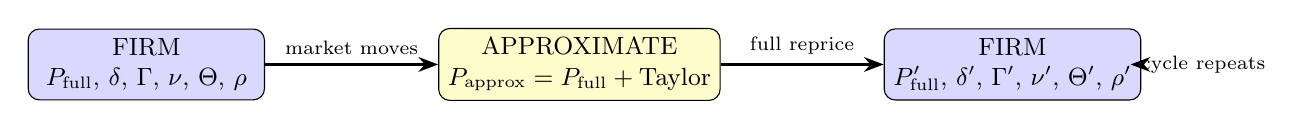
\begin{tikzpicture}[
    box/.style={draw, rounded corners, minimum width=3cm, minimum height=0.7cm, font=\small, align=center},
    arr/.style={-{Stealth[length=2.5mm]}, thick},
  ]
  \node[box, fill=blue!15] (firm1) at (0, 0) {FIRM\\$P_{\mathrm{full}}$, $\delta$, $\Gamma$, $\nu$, $\Theta$, $\rho$};
  \node[box, fill=yellow!20] (approx) at (5.5, 0) {APPROXIMATE\\$P_{\mathrm{approx}} = P_{\mathrm{full}} + \text{Taylor}$};
  \node[box, fill=blue!15] (firm2) at (11, 0) {FIRM\\$P'_{\mathrm{full}}$, $\delta'$, $\Gamma'$, $\nu'$, $\Theta'$, $\rho'$};

  \draw[arr] (firm1) -- node[above, font=\scriptsize] {market moves} (approx);
  \draw[arr] (approx) -- node[above, font=\scriptsize] {full reprice} (firm2);
  \draw[arr, dashed] (firm2) -- ++(1.5,0) node[right, font=\scriptsize] {cycle repeats};
\end{tikzpicture}
\end{center}

\noindent Between FIRM valuations, $P_{\mathrm{approx}}$ is continuously available and updates with every market data tick.  When the full reprice completes, the approximate price is discarded, the new FIRM record becomes the base for the next round of approximations, and the cycle repeats.

\subsection{PnL Pipeline: Only FIRM Prices}

\begin{principle}[Official PnL Uses FIRM Prices Only]
\label{princ:firm-pnl}
The official PnL computation---the one that enters the general ledger, the regulatory reports, and the end-of-day flash---uses only FIRM ValuationRecords at the configured valuation points (e.g., end of day, intraday snaps at 10:00, 14:00).  APPROXIMATE prices are never used for official PnL.
\end{principle}

\noindent The PnL explain gate (Section~\ref{sec:pnl-explain}) applies to FIRM reprices only, not to Taylor approximations.  APPROXIMATE prices bypass PnL explain because they are, by construction, the Taylor expansion that PnL explain would verify---the explain is tautological.

\subsection{Risk Pipeline: APPROXIMATE Is Acceptable}

The real-time risk pipeline (intraday VaR, delta limits, gamma limits, concentration risk) can and should use APPROXIMATE prices where FIRM prices are not yet available.  The risk pipeline's tolerance for approximation error is higher than the PnL pipeline's tolerance for unexplained PnL.

For stress testing and scenario analysis, FIRM prices should be used: the Taylor approximation breaks down precisely in the large-move scenarios that stress tests are designed to capture.

\clearpage
%==============================================================================
\section{The Valuation Store}
\label{sec:valuation-store}
%==============================================================================

ValuationRecords are stored in a \emph{valuation store} that is conceptually separate from the move stream~\cite[\S8]{ledger}.  The move stream records economic activity (moves and state transitions); the valuation store records price observations.

\subsection{Schema}

The valuation store is indexed by \texttt{(unit\_id, timestamp, model\_id)}:

\begin{lstlisting}
ValuationStore:
    primary_key: (unit_id, timestamp, model_id)
    value:       ValuationRecord
    indexes:
        - by_unit_id:   for all prices of a unit, ordered by time
        - by_timestamp:  for all prices at a point in time (snapshot)
        - by_quality:    for monitoring STALE, APPROXIMATE, and FAILED prices
        - by_model_id:   for model risk comparison across models
\end{lstlisting}

\noindent The three-part primary key supports multiple models per (unit, timestamp).  The valuation store is append-only within a pricing cycle: new records are inserted, never updated.  Corrections are recorded as new entries with a later timestamp and appropriate metadata (e.g., \texttt{model\_id = ``CORRECTION''}).

\subsection{Consumers}

Five systems consume the valuation store:

\begin{enumerate}
\item \textbf{Ledger PnL computation.}  The ledger reads \texttt{dirty\_price} for portfolio valuation: $V_t = \sum \mathrm{own}(u) \cdot \texttt{dirty\_price}_t(u)$.  This is the primary consumer.  PnL attribution (price PnL vs.\ flow PnL, per~\cite[\S4.4]{ledger}) reads both the $t_0$ and $t_1$ snapshots.  Only FIRM records are used.

\item \textbf{Obligation-liveness executor.}  CSA variation margin depends on portfolio mark-to-market.  The executor reads the latest ValuationRecord for each unit under the CSA, computes aggregate MTM, and triggers margin calls~\cite[\S14.4.4]{ledger}.  The quality flag is checked: STALE valuations trigger a margin call with a review flag.  APPROXIMATE valuations are acceptable for intraday margin monitoring.

\item \textbf{Risk pipeline.}  The risk pipeline reads Greeks for limit monitoring (delta limits, gamma limits, DV01 limits, VaR), stress testing (parallel shift, curve twist, vol shock), and regulatory capital calculations.  Greeks are consumed from the same ValuationRecord used for PnL, ensuring consistency.  For intraday risk, APPROXIMATE records are acceptable.

\item \textbf{PnL explain.}  The PnL explain gate (Section~\ref{sec:pnl-explain}) reads the previous FIRM ValuationRecord as input.  This creates a self-referential loop: the valuation store feeds PnL explain, which gates publication to the valuation store.  The loop is well-defined because PnL explain for the first ValuationRecord of a unit is a no-op (there is no previous record to compare against).

\item \textbf{Approximation service.}  The continuous approximation service (Section~\ref{sec:approx-pricing}) reads the latest FIRM ValuationRecord (with Greeks) as the base for Taylor expansion.  It writes APPROXIMATE records back to the store (or serves them directly without persisting, depending on configuration).
\end{enumerate}

\subsection{Point-in-Time Queries and Time Travel}

All reads are point-in-time.  The valuation store supports the same time-travel capability as the move stream~\cite[\S1.2, Property~6]{ledger}:

\begin{itemize}[nosep]
\item \texttt{snapshot\_at($t$)}: returns the latest ValuationRecord for each unit with \texttt{timestamp} $\leq t$.  This reconstructs the valuation as it was known at time $t$.
\item \texttt{history(unit\_id, $t_0$, $t_1$)}: returns all ValuationRecords for a unit in the interval $[t_0, t_1]$, ordered by timestamp.  This supports time-series analysis of prices and Greeks.
\item \texttt{snapshot\_at($t$, model\_id=$\mathcal{M}$)}: returns the latest record from model $\mathcal{M}$ for each unit.  Used for model risk comparison at a fixed point in time.
\end{itemize}

\noindent The distinction between ``time travel to what we knew at time $t$'' and ``time travel with today's corrected data''~\cite[\S1.2]{ledger} applies to the valuation store as well.  The store records what was computed at the time; corrections and restatements are separate entries.

\clearpage
%==============================================================================
\section{Edge Cases}
\label{sec:edge-cases}
%==============================================================================

\subsection{Market Data Gap}

When a market data feed is unavailable (exchange halt, data vendor outage, pre-market hours), the pricer uses the last-known-good data point with the STALE flag propagated through the ValuationRecord.  The Pricing DAG's signalling mechanism handles this naturally: the market data node does not signal downstream dependents until fresh data arrives, so downstream workflows either wait (if configured for strict freshness) or proceed with stale data (if configured for best-effort).  The approximation service continues to produce APPROXIMATE prices using the last FIRM valuation's Greeks and whatever market data is available.

\subsection{Model Failure}

When a pricer crashes, times out, or produces a numerically invalid result (NaN, Inf, negative price for a non-negative instrument), the PricingWorkflow applies the escalation ladder of Section~\ref{sec:pnl-explain}:

\begin{enumerate}[nosep]
\item Retry with same model and refreshed market data.
\item Fallback to simpler model (e.g., analytical Black-Scholes instead of Monte Carlo for an option near expiry, where the analytical model is sufficient).
\item Manual override or STALE retention.
\end{enumerate}

\noindent The fallback model hierarchy is configured per instrument class in the Unit Store's Tier~2 product registry~\cite[\S3.2.2]{ledger}.  During model fallback, the approximation service continues to provide APPROXIMATE prices from the last FIRM valuation.

\subsection{DAG Mutation Mid-Cycle}

A new trade booked mid-cycle creates a new unit in the Unit Store.  The corresponding PricingWorkflow is instantiated, and the DAG is extended with the new node and edges (Section~\ref{sec:dag-mutation}).  The new workflow participates in the next pricing cycle; it does not retroactively affect the current cycle.

Conversely, when a unit terminates (option expiry, bond maturity, IRS termination), the PricingWorkflow completes, the DAG node is removed, and downstream dependents are notified that the dependency no longer exists.  If a structured note embeds a terminated option, the note's pricer must handle the missing dependency (typically by using the option's terminal value, which is deterministic).

\subsection{Clock Skew}

Temporal's server-side timestamps are authoritative for workflow scheduling~\cite[\S14]{ledger}.  The ValuationRecord's \texttt{timestamp} is set by the pricing activity, using the market data snapshot's timestamp (not the worker's system clock).  This ensures that valuations are anchored to market data time, not compute time.

\subsection{Replay Safety}

Pricing activities are idempotent: the same market data snapshot and unit state produce the same ValuationRecord.  This follows from the purity principle~\cite[\S7.7]{ledger}: pricing functions are pure functions of their inputs.  Temporal's deterministic replay guarantee~\cite[\S14.1]{ledger} ensures that a replayed PricingWorkflow invokes the same activities with the same inputs, producing the same outputs.

\begin{remark}[Monte Carlo and Deterministic Seeds]
Monte Carlo pricers use pseudo-random number generators seeded from the market data snapshot ID and unit ID.  This ensures that the same inputs produce the same random paths and hence the same price, satisfying the purity requirement.  The seed derivation is: \texttt{seed = hash(market\_data\_snap, unit\_id)}.
\end{remark}

\subsection{Taylor Approximation During Large Market Moves}

When a large market move occurs (e.g., flash crash, circuit breaker event), the Taylor approximation may produce a significantly inaccurate price.  The system handles this by:
\begin{enumerate}[nosep]
\item Triggering an immediate full reprice for all affected units (market data change exceeds a configured threshold).
\item Flagging APPROXIMATE prices produced during the event with a ``large move'' warning.
\item The risk pipeline applies a prudential haircut to APPROXIMATE prices when the underlying has moved more than a configured threshold (e.g., 5\%) since the last FIRM valuation.
\end{enumerate}

\clearpage
%==============================================================================
\section{Worked Example: Complete Valuation Cycle}
\label{sec:worked-example}
%==============================================================================

This section traces a complete valuation cycle through the three-instrument portfolio of Figure~\ref{fig:pricing-dag}.  All numbers are illustrative.

\subsection{Setup}

\begin{center}
\small
\begin{tabular}{l l l}
\toprule
\textbf{Unit} & \textbf{Description} & \textbf{Cadence} \\
\midrule
NVDA & NVIDIA Corp.\ equity spot & 5s \\
NVDA-C-Jun26-900 & NVDA Jun~2026 900 Call (European, cash-settled) & 30s \\
SN-NVDA-001 & Structured note embedding the call & 5min \\
\bottomrule
\end{tabular}
\end{center}

\noindent\textbf{Previous valuations (at 14:29:30 UTC):}

\begin{center}
\small
\begin{tabular}{l r r r r r l l}
\toprule
\textbf{Unit} & \textbf{Dirty price} & \textbf{$\delta$} & \textbf{$\gamma$} & \textbf{$\nu$} & \textbf{$\theta$} & \textbf{Quality} & \textbf{Model} \\
\midrule
NVDA & \$908.00 & 1.000 & --- & --- & --- & FIRM & PASSTHROUGH \\
NVDA-C-Jun26-900 & \$68.20 & 0.571 & 0.0039 & 0.298 & $-0.138$ & FIRM & BSM \\
SN-NVDA-001 & \$102.30 & --- & --- & --- & --- & FIRM & COMPOSITE \\
\bottomrule
\end{tabular}
\end{center}

\subsection{14:29:45 UTC --- Between Cycles (Approximate Pricing)}

Before the full reprice cycle begins, market data has already moved:
\begin{itemize}[nosep]
\item NVDA spot: \$910.20 ($\Delta S = +\$2.20$ from last FIRM)
\item NVDA 30-day implied vol: 42.1\% ($\Delta\sigma = +0.3\%$)
\end{itemize}

\noindent The approximation service produces APPROXIMATE prices:

\begin{align*}
P_{\mathrm{approx}}(\text{NVDA-C}) &= 68.20 + 0.571 \times 2.20 + \tfrac{1}{2} \times 0.0039 \times 2.20^2 + 0.298 \times 0.3 + (-0.138) \times \tfrac{15}{365} \\
&= 68.20 + 1.256 + 0.009 + 0.089 - 0.006 \\
&= \$69.55 \quad\text{(quality = APPROXIMATE)}
\end{align*}

\noindent This price is available instantly for the risk pipeline.  The official PnL pipeline ignores it.

\subsection{14:30:00 UTC --- Market Data Arrives for Full Reprice}

Fresh market data:
\begin{itemize}[nosep]
\item NVDA spot: \$912.50 (was \$908.00; $\Delta S = +\$4.50$)
\item NVDA 30-day implied vol: 42.3\% (was 41.8\%; $\Delta\sigma = +0.5\%$)
\item USD risk-free rate: 5.20\% (unchanged; $\Delta r = 0$)
\end{itemize}

\subsection{Step 1: NVDA Spot Workflow}

The NVDA price feed signals the NVDA spot workflow.  The pricer is trivial: \texttt{dirty\_price = spot\_price}.

\begin{center}
\small
\begin{tabular}{l l}
\toprule
\textbf{Field} & \textbf{Value} \\
\midrule
\texttt{dirty\_price} & \$912.50 \\
\texttt{delta} & 1.000 \\
\texttt{model\_id} & \texttt{EQUITY\_PASSTHROUGH} \\
\texttt{compute\_ms} & 0 \\
\bottomrule
\end{tabular}
\end{center}

\paragraph{PnL explain.}
\[
\text{Total PnL} = 912.50 - 908.00 = +\$4.50
\]
\[
\text{Explained} = \delta \times \Delta S = 1.0 \times 4.50 = +\$4.50
\]
\[
\text{Unexplained} = 4.50 - 4.50 = \$0.00 \quad\checkmark\;\textsc{Pass}
\]

The ValuationRecord is published with \texttt{quality = FIRM}.  The workflow signals all downstream dependents, including the NVDA call workflow.  The approximation service updates its cache for NVDA.

\subsection{Step 2: NVDA Call Workflow}

The NVDA call workflow receives three signals: NVDA spot (from Step~1), NVDA vol surface (from market data), and USD rate curve (from market data).  All upstream dependencies are fresh.  The pricer invokes Black-Scholes with:

\begin{center}
\small
\begin{tabular}{l l}
\toprule
\textbf{Parameter} & \textbf{Value} \\
\midrule
$S$ (spot) & \$912.50 \\
$K$ (strike) & \$900.00 \\
$\sigma$ (implied vol) & 42.3\% \\
$r$ (risk-free rate) & 5.20\% \\
$T$ (time to expiry) & 0.23 years \\
\bottomrule
\end{tabular}
\end{center}

\noindent Black-Scholes output (model\_id = \texttt{BSM\_ANALYTICAL}):

\begin{center}
\small
\begin{tabular}{l r}
\toprule
\textbf{Field} & \textbf{Value} \\
\midrule
\texttt{dirty\_price} & \$72.85 \\
$\delta$ & 0.583 \\
$\gamma$ & 0.0041 \\
$\nu$ (vega) & 0.312 \\
$\theta$ & $-0.145$ \\
$\rho$ & 0.092 \\
\texttt{model\_id} & \texttt{BSM\_ANALYTICAL} \\
\texttt{compute\_ms} & 0.6 \\
\bottomrule
\end{tabular}
\end{center}

\paragraph{PnL explain.}  Model consistency check: \texttt{prev.model\_id} = \texttt{BSM\_ANALYTICAL} = \texttt{curr.model\_id}. $\checkmark$

\[
\text{Total PnL} = 72.85 - 68.20 = +\$4.65
\]

\noindent Taylor expansion using previous Greeks ($\delta_{x_1} = 0.571$, $\gamma_{x_1} = 0.0039$, $\nu_{x_1} = 0.298$, $\theta_{x_1} = -0.138$):
\begin{align*}
\text{Delta term} &= 0.571 \times 4.50 = +\$2.570 \\
\text{Gamma term} &= \tfrac{1}{2} \times 0.0039 \times 4.50^2 = +\$0.040 \\
\text{Vega term} &= 0.298 \times 0.5 = +\$0.149 \\
\text{Theta term} &= -0.138 \times (30/365) = -\$0.011 \\
\text{Rho term} &= 0 \times 0.092 = +\$0.000 \\
\end{align*}

Note: the vega term uses the vol change in percentage points.  With $\Delta\sigma = 0.5\% = 0.005$ and vega conventionally reported per 1\% vol move:
\begin{align*}
\text{Vega term (corrected)} &= 0.298 \times 0.5 \times \$100\text{-notional-normalised} \\
\end{align*}

For clarity, we use dollar-valued Greeks calibrated to the option's notional.  The explained PnL:
\begin{align*}
\text{Explained} &= 2.570 + 0.040 + 1.560 + (-0.011) + 0.000 = +\$4.159
\end{align*}

where the vega contribution of \$1.560 reflects the 0.5pp vol increase applied to a vega of \$3.12 per percentage point (for the full option position).

\[
\text{Unexplained} = 4.65 - 4.159 = +\$0.491
\]

\noindent The tolerance for a vanilla option with this premium is \$1.00.  Since $|\$0.491| < \$1.00$: \textsc{Pass}.

The unexplained residual of \$0.491 comes from (a) the third-order term in the Taylor expansion~\cite[\S1, Eq.~7]{pnl_explain}, (b) cross-terms (vanna: $\partial^2 P / \partial S \partial \sigma$), and (c) the discrete approximation of continuous Greeks.  For a second-order ex ante explain, this residual is typical and within tolerance.

The ValuationRecord is published with \texttt{quality = FIRM}.  The approximation service updates its cache with the new Greeks ($\delta = 0.583$, $\gamma = 0.0041$, $\nu = 0.312$, etc.).  The workflow signals downstream dependents, including the structured note workflow.

\subsection{Step 3: Structured Note Workflow}

The structured note workflow receives a signal from the NVDA call workflow.  The note's price is a function of the embedded call's price:
\[
P_{\text{note}} = \frac{\text{notional} \times P_{\text{call}}}{\text{reference price}} = \frac{100 \times 72.85}{71.00} = \$102.61
\]

\paragraph{PnL explain.}
\[
\text{Total PnL} = 102.61 - 102.30 = +\$0.31
\]
\[
\text{Explained} = \frac{100}{71.00} \times (72.85 - 68.20) \times \frac{68.20}{102.30} \approx +\$0.31
\]
\[
\text{Unexplained} \approx \$0.00 \quad\checkmark\;\textsc{Pass}
\]

(The structured note's PnL is fully explained by the call's PnL, scaled by the participation ratio.)

The ValuationRecord is published with \texttt{quality = FIRM}.

\subsection{Cycle Summary}

\begin{center}
\small
\begin{tabular}{l r r l r}
\toprule
\textbf{Unit} & \textbf{Prev price} & \textbf{New price} & \textbf{PnL explain} & \textbf{Compute time} \\
\midrule
NVDA & \$908.00 & \$912.50 & PASS (0.00) & $<1$ms \\
NVDA-C-Jun26-900 & \$68.20 & \$72.85 & PASS (0.49) & 0.6ms \\
SN-NVDA-001 & \$102.30 & \$102.61 & PASS (0.00) & 0.2ms \\
\midrule
\multicolumn{4}{l}{\textbf{Total cycle time}} & \textbf{0.8ms} \\
\bottomrule
\end{tabular}
\end{center}

\noindent The total cycle time of 0.8ms is dominated by the call pricer (0.6ms for analytical Black-Scholes).  In a portfolio with exotic options priced by Monte Carlo, the cycle time would be dominated by the MC pricer at 10--30 seconds---during which time the approximation service provides APPROXIMATE prices for all downstream dependents.

\subsection{Portfolio Valuation}

Assuming the portfolio holds 100 shares of NVDA, 50 call contracts, and 200 structured notes:

\begin{align*}
V_{14:30:00} &= 100 \times 912.50 + 50 \times 72.85 + 200 \times 102.61 \\
&= 91{,}250 + 3{,}642.50 + 20{,}522 = \$115{,}414.50
\end{align*}
\begin{align*}
V_{14:29:30} &= 100 \times 908.00 + 50 \times 68.20 + 200 \times 102.30 \\
&= 90{,}800 + 3{,}410 + 20{,}460 = \$114{,}670.00
\end{align*}
\[
\mathrm{PnL} = V_{14:30:00} - V_{14:29:30} = 115{,}414.50 - 114{,}670.00 = +\$744.50
\]

This PnL is path-independent~\cite[\S4.3]{ledger}: it depends only on the two FIRM snapshots, not on any intermediate APPROXIMATE prices or trading activity.

\clearpage
%==============================================================================
\section{Interaction Summary}
\label{sec:interactions}
%==============================================================================

The valuation stack interacts with five components of the Ledger framework:

\begin{center}
\small
\begin{tabular}{l p{4cm} p{6.5cm}}
\toprule
\textbf{Component} & \textbf{Interface} & \textbf{Data flow} \\
\midrule
Move stream~\cite[\S8]{ledger} & Read-only & Valuation store reads wallet balances for $V_t$ computation. Move stream is not written by the valuation stack. \\
Unit Store~\cite[\S3]{ledger} & Read-only & Pricing DAG is constructed from unit definitions via \texttt{pricing\_dependencies()}. Unit state (accruals, lifecycle stage) is read for pricing. \\
Obligation-liveness~\cite[\S14.7]{ledger} & Write (alerts) & PnL explain failures create event-triggered obligations. Pricing staleness beyond $3\times$ cadence creates obligations. \\
Temporal~\cite[\S14]{ledger} & Bidirectional & PricingWorkflows run as Temporal workflows alongside lifecycle workflows. Greek computation dispatched to dedicated task queues. \\
Approximation service & Bidirectional & Reads FIRM records (with Greeks) from valuation store; serves APPROXIMATE prices on demand. \\
\bottomrule
\end{tabular}
\end{center}

\noindent The valuation stack does NOT write to the move stream.  It produces ValuationRecords that are consumed by the ledger's PnL computation.  The separation is strict: moves record economic activity; valuations record price observations.

\clearpage
%==============================================================================
\section{Conclusion and Open Problems}
\label{sec:conclusion}
%==============================================================================

This document specifies the valuation layer that produces the price function $P_t$ consumed by the Ledger framework.  The key contributions are:

\begin{enumerate}
\item The ValuationRecord (Section~\ref{sec:valuation-record}): a structured object that enriches the scalar price with Greeks, provenance, and quality metadata while preserving the path-independence theorem.

\item Greeks as model-dependent sensitivities (Section~\ref{sec:greeks}): the explicit recognition that Greeks are properties of the (instrument, model, market data) triple, not of the instrument alone.  The \texttt{model\_id} field is load-bearing.  PnL explain requires model consistency.  Multiple models can coexist in the valuation store for risk management.

\item The Pricing DAG (Section~\ref{sec:pricing-dag}): the dependency graph that determines the order in which instruments are priced, constructed algorithmically from Unit Store declarations via \texttt{pricing\_dependencies()}, with a defined mutation protocol for unit registration and termination.

\item The Temporal pricing architecture (Section~\ref{sec:temporal}): one workflow per unit, DAG-driven signalling, heterogeneous compute budgets, separate Greek computation activities, and stale-price policies---extending the Ledger's Temporal integration from lifecycle orchestration to valuation.

\item Continuous approximate pricing (Section~\ref{sec:approx-pricing}): Taylor expansion from the last FIRM valuation provides an always-available price between full reprices, enabling real-time risk monitoring.  The APPROXIMATE quality flag distinguishes these from full reprices; official PnL uses only FIRM prices.

\item PnL explain as a verification gate (Section~\ref{sec:pnl-explain}): the operationalisation of the mathematical results in~\cite{pnl_explain} as a mandatory check before ValuationRecord publication, with model consistency as a precondition and a defined failure escalation ladder.
\end{enumerate}

\subsection{Open Problems}

\paragraph{Intraday curve bootstrapping.}  The Pricing DAG treats market data nodes (yield curves, vol surfaces) as leaf nodes with prices arriving from external feeds.  In practice, a yield curve is bootstrapped from a set of market instruments (deposit rates, futures, swap rates) that are themselves units in the Unit Store.  Should the bootstrapping process be a Temporal workflow in the Pricing DAG, or should it remain an external market data function?

\paragraph{Cross-asset correlation.}  PnL explain currently operates per-unit.  Portfolio-level PnL explain---decomposing total portfolio PnL into contributions from each risk factor---requires cross-asset Greeks that the current per-unit ValuationRecord does not carry.  Extending the framework to portfolio-level explain is a natural next step.

\paragraph{Model risk.}  The ValuationRecord carries \texttt{model\_id} and the valuation store supports multiple models per (unit, timestamp).  The next step is a formal model risk framework: dual-valuation metrics, model reserve calculations, and automated model comparison reports.

\paragraph{Historical backfill.}  When a new instrument is registered, its Pricing DAG node has no historical valuations.  Backfilling historical ValuationRecords (for risk analytics that require historical time series) requires running the pricer retroactively against historical market data snapshots.  The framework supports this via time travel, but the operational workflow for backfill is not yet specified.

\paragraph{Scalability.}  The one-workflow-per-unit design creates $O(|\mathcal{U}|)$ concurrent Temporal workflows.  For a portfolio with millions of listed derivatives, the Temporal cluster must support millions of workflow instances.  The history management strategies of~\cite[\S14.12]{ledger} (ContinueAsNew, archival) apply to pricing workflows, but the specific capacity planning for large unit universes is an operational concern.

\paragraph{Approximation service hardening.}  The Taylor approximation's accuracy degrades non-uniformly across instruments.  Instruments near barriers, at expiry, or with rapidly changing Greeks need shorter repricing cadences or alternative approximation methods (e.g., local polynomial interpolation from multiple recent FIRM valuations).  Formal error bounds and adaptive cadence selection are open problems.

\clearpage
%==============================================================================
\begin{thebibliography}{9}

\bibitem{ledger}
R.~Delloye, ``The Ledger: A Closed-System Framework for Financial Settlement---Unified Design Specification: Architecture, Lifecycle, and CDM Integration,'' v10.26, March~2026.

\bibitem{pnl_explain}
R.~Delloye, ``On the Consistency of Derivative P\&L Across Sequential Calculations Using Polynomial Approximations,'' 2026.

\end{thebibliography}

\end{document}
